\documentclass[a4paper,11pt]{article}
\pagestyle{headings}

\usepackage[utf8]{inputenc}
\usepackage[french]{babel}
\usepackage{graphicx}
\usepackage{float}
\usepackage{diagbox}
\usepackage[T1]{fontenc}
\graphicspath{{images/}}

\title{Rapport du projet 1 de reconnaissance faciale}
\author{Auriane Reverdell, Felix Hähnlein, Romain Duléry}
\date{\today}

\setlength{\oddsidemargin}{0.2cm}
\setlength{\evensidemargin}{-0.7cm}
\setlength{\parindent}{30pt}
\setlength{\textwidth}{15cm}
\setlength{\textheight}{24cm}
\setlength{\topmargin}{-.5in}
\setlength{\parskip}{1ex}

\begin{document}

\maketitle
\vspace{1cm}

\section{Résumé du travail réalisé}
\section{Analyse des résultats expérimentaux}
\subsection{Phase d'apprentissage}

\subsubsection{Travail réalisé}

La phase d'apprentissage consiste en la création de la Lookup Table, qui associe à chaque couleur une probabilité d'appartenance à la cible, ici à la peau.

3 paramètres entrent en jeu :

\begin{itemize}
    \item La dataset utilisée
    \item La quantification des couleurs N
    \item L'espace de couleur utilisé\\
\end{itemize}

Nous avons implémenté l'utilisation des espaces de couleur RGB et RG (chrominances). Nous avons utilisé l'outil PyQTGraph afin de visualiser les Lookup Tables en 3 dimensions, avec chaque couleur représentée par une sphère, dont la taille est proportionnelle à la probabilité de correspondance à de la peau.\\

Voici des exemples de résultats obtenus :

\begin{figure}[H]
\begin{center}
    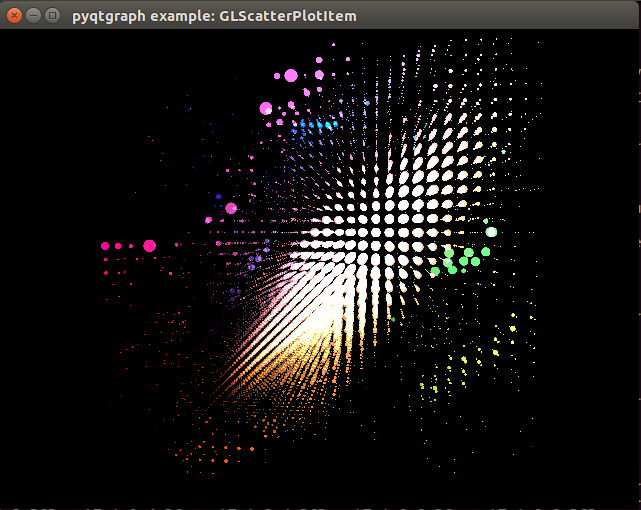
\includegraphics[scale=0.5]{lT_1_9_8_RGB.png}
    \caption{Lookup Table obtenue avec les fichiers 1 à 9, N=32 couleurs, en RGB}
\end{center}
\end{figure}

\begin{figure}[H]
\begin{center}
    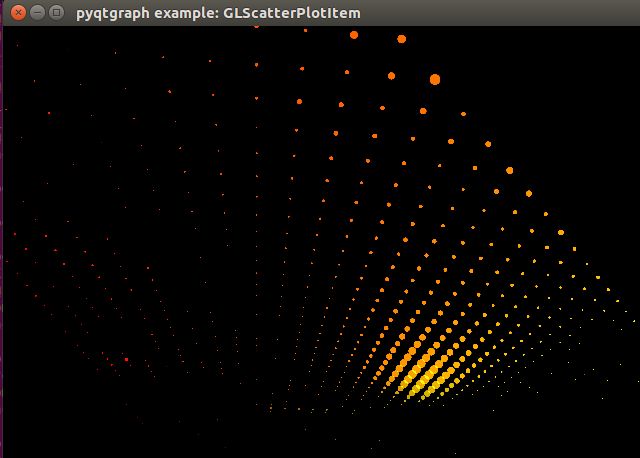
\includegraphics[scale=0.5]{lT_1_9_4_RG.png}
    \caption{Lookup Table obtenue avec les fichiers 1 à 9, N=64 couleurs, en RG}
\end{center}
\end{figure}

On constate que dans les deux cas, les couleurs prédominantes correspondent bien à de potentielles couleurs de peau.

\subsubsection{Analyse de l'influence des paramètres}

Nous avons utilisé l'aire sous les courbes ROC en guise de méthode d'évaluation.

Voici les résultats obtenus pour les 100 premières images du fichier 10, avec différents paramètres :

\begin{itemize}
    \item En utilisant l'espace de couleur RGB\\

        \begin{center}
            \begin{tabular}{| c | p{2cm} | p{2cm} | p{2cm} | p{2cm} |}
                \hline
                \diagbox{Data}{N} & 128 & 64 & 32 & 16 \\
                \hline
                2 & 0.8446 & 0.8570 & 0.8639 & 0.8655 \\
                9 & 0.8634 & 0.8687 & \textbf{0.8702} & 0.8682 \\
                \hline
            \end{tabular}
        \end{center}~\\

    \item En utilisant l'espace de couleur RG\\

        \begin{center}
            \begin{tabular}{| c | p{2cm} | p{2cm} | p{2cm} | p{2cm} |}
                \hline
                \diagbox{Data}{N} & 128 & 64 & 32 & 16 \\
                \hline
                2 & 0.8626 & 0.8620 & 0.8591 & 0.8555 \\
                9 & \textbf{0.8630} & 0.8622 & 0.8580 & 0.8550 \\
                \hline
            \end{tabular}
        \end{center}

\end{itemize}~\\

Data désigne le dernier fichier utilisé pour l'entrainement : dans le cas où Num fichier vaut 2, les images des fichiers 01 et 02 ont été utilisées pour l'entrainement.

Tout d'abord, les meilleurs résultats obtenus l'ont été avec l'entrainement sur 9 fichiers, N = 32, et en espace RGB, mais il y a peu de différence de performances en fonction des paramètres.

On peut toutefois relever certaines informations.

Au niveau de la quantification, on constate que les meilleurs résultats sont obtenus avec N = 32 en RGB et N = 128 en RG. On peut conjecturer qu'en RG, étant donné qu'on stocke beaucoup moins d'informations, on a besoin que celles-ci soient plus précises.

Au niveau de la dataset, en RGB il est notable qu'il est préférable d'entrainer l'algorithme autant que possible. Toutefois celle-ci est suffisamment pertinente et bien 'mélangée' pour que cette influence soit faible.

Enfin, il n'y a pas de différence notable d'aspect entre les différences courbes ROC obtenues.

En voici une à titre d'exemple :

\begin{figure}[H]
\begin{center}
    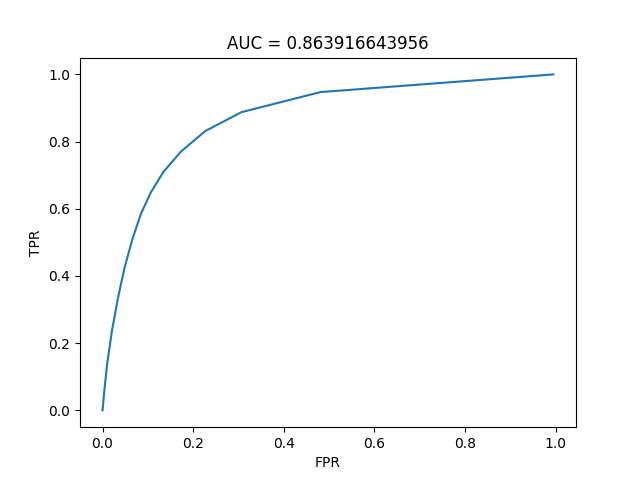
\includegraphics[scale=0.5]{ROC_8_RGB.png}
    \caption{Courbe ROC obtenue avec les fichiers 1 et 2, N=32 couleurs, en RGB}
\end{center}
\end{figure}

\subsection{Détection faciale}

La phase de la détection faciale est différente de celle de la phase d'apprentissage. 
Alors qu'avant on s'intéressait à la construction de la table de probabilité la plus fiable pour détecter de la peau humaine, dans cette partie, il s'agit d'exploiter cette information afin de pouvoir donner en sortie un ensemble de formes qui englobent des éventuels visages.\\
\newline
Nous nous sommes intéressés à deux approches bien distinctes d'utiliser ce \og détecteur de peau humaine\fg{}. 
La première va chercher à trouver directement les visages à l'intérieur des ROI pendant que la deuxième va utiliser les ROI comme un système de filtrage et essayer de reconstruire les visages grâce à sa sortie.
\newline
\subsubsection{Détection de visage sans post-traitement}
Cette technique vise à fournir les visages en sortie directement après les avoir détecté dans une zone d'intérêt.
Cela semble être intuitif, elle est même la principale raison pour laquelle nous les avons introduit.
Néanmoins, la principale difficulté que nous avons rencontré avec cette approche est le choix de la taille de la ROI.
Encore une fois, il semble y avoir deux stratégies pour trouver une taille convenable.\\
\newline
Premièrement, on peut l'intuiter à partir des dimensions de l'image où en moyennant les tailles rencontrées pendant la phase d'apprentissage.
Cette stratégie a l'avantage qu'elle est facile à implémenter, mais elle ne va pas fournir des résultats satisfaisants, car en réalité, l'aire occupée par un visage peut varier fortement.
Il suffit de prendre comme exemple une image de portrait et une image qui contient un visage dans l'arrière-plan.\\
\newline
Deuxièmement, on peut utiliser des ROI de taille adaptative. 
Cette stratégie va faire agrandir la zone dans une certaine direction tant que le critère d'arrêt n'a pas été rempli.
Un exemple de critère d'arrêt utilisé par d'autres systèmes est la décroissance de la probabilité accumulée au sein d'une ROI.
Cela correspond au dépassement de la région faciale, mais il s'avère que son défaut principal est le rejet des parties de visages n'ayant pas une couleur similaire à celle de la peau humaine, comme par exemple les yeux, les lunettes, une bouche ouverte, etc.
\newline
\newline
En poursuivant une de ces deux stratégies avec une ROI rectangulaire, il est pertinent d'utiliser un filtre gaussien pour tenir compte de la forme elliptique de la partie anatomique visée.
RESULTATS
\subsubsection{Détection de visage avec post-traitement}
Pour contourner le problème précédemment décrit, on peut envisager d'agglomérer les détections positives fournies par le système de filtrage des ROI.
En faisant ceci, on n'utilise les ROI que pour connaître la probabilité d'une zone de l'image de faire partie de la peau humaine.
D'ailleurs, cette interprétation correspond exactement à la manière dont on a construit la table de probabilités pendant la première phase.
\newline
\newline
L'algorithme de partitionnement de données (en angl. {\textit{clustering}}) choisi est l'algorithme espérance-maximisation.
Il s'agit d'un algorithme largement utilisé dans le domaine de l'apprentissage automatique dont le principal avantage pour notre application par rapport à l'algorithme k-means est l'utilisation de l'espérance au lieu d'une norme spatiale pour décider l'attribution à un certain cluster.
L'algorithme k-means va donc favoriser des clusters sphériques, alors que l'algorithme EM permet des formes elliptiques quelconques, ce qui est avantageux pour reconstruire des visages.\\
\newline
Nous avons rencontré deux principales difficultés avec cet algorithme. 
Pour l'initialiser, il faut préciser le nombre de clusters qu'on cherche à construire et des visages spatialement proches vont être reconnus comme provenant d'une même personne.
Le premier problème revient à un problème d'ajustement de modèle. On ne veut pas surajuster ni sous-ajuster le nombre de paramètres utilisés pour décrire les données.
Une méthode communément utilisée pour trouver le meilleur paramétrage est l'utilisation d'un critère d'information bayésien.
Ce critère se base sur un calcul de probabilité faisant intervenir la vraisemblance du modèle choisi, le nombre de paramètres utilisés et le nombre de données en entrée.
En pratique, nous évaluons le modèle pour un intervalle de paramètres et choisissons ensuite le paramètrage qui a obtenu un critère minimal.
\newline
\newline
Pour résoudre le problème des visages proches, nous proposons d'appliquer le clustering non seulement aux données spatiales, mais également aux données chromatiques.
En effet, en supposant que les détections positives qui ont une même couleur proviennent de la même personne, nous pouvons faire la distinction entre des personnes spatialement proches.
\newline
\newline
Une autre application possible du partitionnement des couleurs est la détection d'une partie du corps qu'on ne veut pas reconnaître, mais qui a une couleur similaire à celle de la peau humaine, comme par exemple une main.

\end{document}
